\documentclass[aspectratio=169]{beamer}
\beamertemplatenavigationsymbolsempty
\usepackage[utf8]{inputenc}
\usepackage[T1]{fontenc}
\usepackage{lmodern}
\usepackage{bm}
\usepackage{amsmath,amssymb}
\usepackage{booktabs}
\usepackage{tikz}
\usetikzlibrary{positioning,arrows.meta,shapes.geometric,calc}
\usepackage{pgfplots}
\pgfplotsset{compat=1.18}
\usepackage{graphicx}
\usepackage{tabularx}
\usepackage{array}
\usepackage{xcolor}
\usepackage{colortbl}
\usepackage{pifont}
\usepackage{makecell}
\usepackage{adjustbox}

% Weekly update, October 7, 2026: the triage classifier that replaces the
% balanced hypothesis screen (GNN arm and LLM arm), the GNN-gated evidence
% profile, its DAgger cell, and the trace review.  Style follows the 16:9
% Madrid/beaver weekly template of October 2.  Sources are on the last slide.
% Build: pdflatex -interaction=nonstopmode -halt-on-error weekly_update_20261007.tex

% ====== Macros ======
\newcommand{\cmark}{\textcolor{green!60!black}{\ding{51}}}
\newcommand{\xmark}{\textcolor{red!70!black}{\ding{55}}}
\newcommand{\good}[1]{\textcolor{green!50!black}{\textbf{#1}}}
\newcommand{\bad}[1]{\textcolor{red!70!black}{\textbf{#1}}}
\newcommand{\warn}[1]{\textcolor{orange!80!black}{\textbf{#1}}}
\newcommand{\code}[1]{\texttt{\detokenize{#1}}}
\newcommand{\tightvspace}{\vspace{0.35em}}
\newcommand{\reportsource}[1]{{\vskip 0.4em\tiny\textcolor{gray!80!black}{\textbf{Source:} #1}\par}}
\newcommand{\scope}[1]{{\small\textit{#1}}\par\vspace{0.4em}}

\newcolumntype{Y}{>{\raggedright\arraybackslash}X}
\newcolumntype{P}[1]{>{\raggedright\arraybackslash}p{#1}}
\newcolumntype{L}[1]{>{\raggedright\arraybackslash}p{#1}}

\usetheme{Madrid}
\usecolortheme{beaver}
\setbeamertemplate{caption}[numbered]
\setlength{\tabcolsep}{4pt}
\renewcommand{\arraystretch}{1.12}
% Beamer's \appendix puts \translate into the PDF bookmarks.
\pdfstringdefDisableCommands{\def\translate#1{#1}}

\tikzset{
  stage/.style={draw=gray!65, rounded corners=2pt, fill=gray!7, align=center,
    inner sep=3pt, minimum height=0.8cm},
  gate/.style={stage, fill=orange!14, draw=orange!60!black},
  phys/.style={stage, fill=blue!7, draw=blue!45!black},
  gnn/.style={stage, fill=violet!8, draw=violet!55!black},
  leak/.style={stage, fill=red!8, draw=red!50!black},
  outc/.style={stage, fill=green!8, draw=green!40!black},
  arr/.style={-{Stealth[length=1.8mm]}, thick, gray!70!black},
  lab/.style={font=\tiny\itshape, fill=white, inner sep=1pt},
}

\title[Power System LLM]{Weekly Report}
\subtitle{Triage Classifier: the GNN Gate and the LLM Arm}
\author{Yifei Xu}
\institute{New York University}
\date{October 7, 2026}

\begin{document}
\maketitle

% 2
\begin{frame}{This Week's Changes}
  \begin{itemize}
    \setlength\itemsep{0.55em}
    \item \textbf{Direction:} replace the balanced hypothesis screen (median 1.1\,s per alarm, 229 refits per round) by a classifier that reads only the balanced WLS solve. Two arms: a graph neural network, and the LLM itself.
    \item \textbf{GNN:} \textbf{100\%} recall with \textbf{0.9\%} unneeded phasor requests in 2\,ms; the screen gets 98.5\% and 12.0\%. No simulator-background effect.
    \item \textbf{LLM as the classifier:} six fine-tunes over three prompt forms; best greedy recall 83\%. Trees on the same prompt fields reach 98.5\%. Closed for IEEE 14.
    \item \textbf{GNN-gated profile:} the rule expert solves \textbf{159/160} development roots in 4.1\,min, the same roots as with the screen in 10\,min.
    \item \textbf{DAgger cell with the GNN gate:} round 1 expert 159, BC0 153, \textbf{R1 159} of 160 (screen cell: 160, 152, 158). Round 2 is in evaluation.
    \item \textbf{Trace review:} no family leak found; four contract changes cut tool calls by 9.4\% at equal success.
  \end{itemize}
\end{frame}

% 3
\begin{frame}{Why Replace the Screen}
  \begin{columns}[T]
    \begin{column}{0.47\textwidth}
      \small
      \textbf{Cost.} After every alarm the screen refits the operator's balanced model under each single cause.
      \begin{center}
        \footnotesize
        \renewcommand{\arraystretch}{1.12}
        \begin{tabular}{lr}
          \toprule
          Class & Refits per round \\
          \midrule
          Meter & 6 \\
          Parameter ($R$, $X$, both) & 60 \\
          Outage & 19 \\
          HIF (16 lines $\times$ 9 positions) & 144 \\
          \midrule
          One round & \textbf{229} \\
          \bottomrule
        \end{tabular}
      \end{center}
      Median \warn{1.1\,s} per alarm against 0.05\,s for the WLS itself, and the count grows with the branch count.
    \end{column}
    \begin{column}{0.5\textwidth}
      \small
      \textbf{The LLM's role.} The agent read the screen's verdict in its prompt, so the LLM never classified anything from the WLS result.
      \par\vspace{0.7em}
      \textbf{Decisions of October 4}\par\vspace{0.2em}
      \footnotesize
      \renewcommand{\arraystretch}{1.18}
      \begin{tabularx}{\linewidth}{L{0.55cm}Y}
        \toprule
        G1 & The classifier's thresholded score gates a request for phase-resolved measurements. \\
        T1 & Labels come from the truth: a request is needed when it holds an HIF, an unbalance or a harmonic source. \\
        S1 & Start with an offline benchmark on IEEE 14; IEEE 57 and 118 later. \\
        \bottomrule
      \end{tabularx}
      \par\vspace{0.5em}
      \small Two arms: a GNN whose score is the gate, and the LLM deciding by itself.
    \end{column}
  \end{columns}
  \reportsource{S1 (sections 1--2), S9 (screen cost, October 2).}
\end{frame}

% 4
\begin{frame}{What the Classifier Decides}
  \small
  \begin{itemize}
    \setlength\itemsep{0.55em}
    \item \textbf{Two decisions.} Request PMU phasors or not, and which balanced family to try first: meter, parameter or topology. Six family scores are a diagnostic only.
    \item \textbf{Labels (T1).} A request is needed when the truth holds an HIF, an unbalance or a harmonic source. On a mixed root, the first family is the one whose removal lowers $J$ most.
    \item \textbf{Not the classifier's job.} Locating the HIF: the zero-sequence line differential on the acquired phasors does that.
    \item \textbf{Fallbacks that need no screen.} Phasors open when every balanced correction on the state was rejected by verification, or none was offered while the alarm stands. Spectra follow phasors that came back balanced.
    \item \textbf{Operating point.} Every learned score is thresholded on the calibration split at the screen rule's recall (99.3\%), so the tables compare unneeded requests at equal recall.
  \end{itemize}
  \reportsource{S1 (sections 2, 3 and 5).}
\end{frame}

% 5
\begin{frame}{GNN Triage Model}
  \begin{center}
  \begin{adjustbox}{max width=\textwidth}
  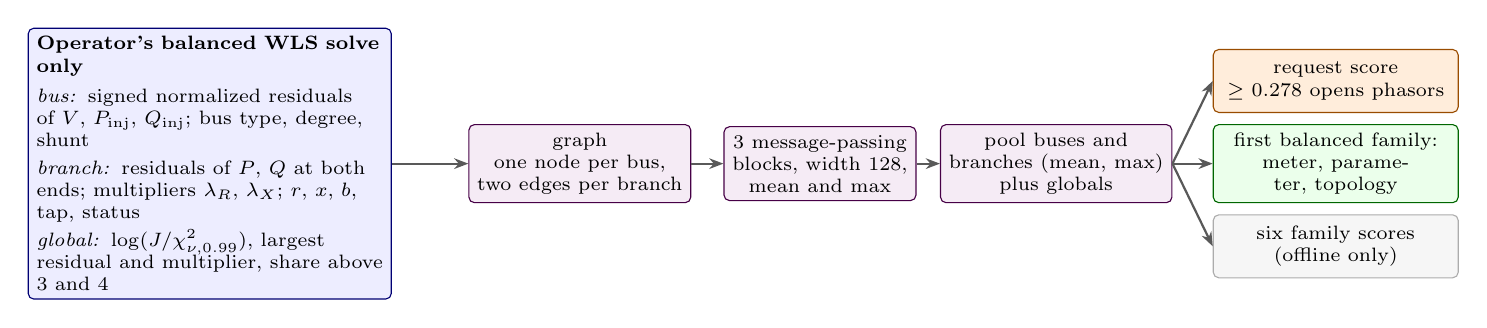
\begin{tikzpicture}[font=\scriptsize]
    \node[phys, text width=4.4cm, align=left] (in) at (0,0) {%
      \textbf{Operator's balanced WLS solve only}\\[3pt]
      \textit{bus:} signed normalized residuals of $V$, $P_{\rm inj}$, $Q_{\rm inj}$; bus type, degree, shunt\\[2pt]
      \textit{branch:} residuals of $P$, $Q$ at both ends; multipliers $\lambda_R$, $\lambda_X$; $r$, $x$, $b$, tap, status\\[2pt]
      \textit{global:} $\log(J/\chi^2_{\nu,0.99})$, largest residual and multiplier, share above $3$ and $4$};
    \node[gnn] (graph) at (4.7,0) {graph\\one node per bus,\\two edges per branch};
    \node[gnn] (mp) at (7.75,0) {3 message-passing\\blocks, width 128,\\mean and max};
    \node[gnn] (pool) at (10.75,0) {pool buses and\\branches (mean, max)\\plus globals};
    \node[gate, text width=2.9cm] (req) at (14.3,1.05) {request score\\$\geq 0.278$ opens phasors};
    \node[outc, text width=2.9cm] (first) at (14.3,0) {first balanced family:\\meter, parameter, topology};
    \node[stage, text width=2.9cm] (fam) at (14.3,-1.05) {six family scores\\(offline only)};
    \draw[arr] (in) -- (graph);
    \draw[arr] (graph) -- (mp);
    \draw[arr] (mp) -- (pool);
    \draw[arr] (pool.east) -- (req.west);
    \draw[arr] (pool.east) -- (first.west);
    \draw[arr] (pool.east) -- (fam.west);
  \end{tikzpicture}
  \end{adjustbox}
  \end{center}
  \footnotesize
  \begin{itemize}
    \setlength\itemsep{0.25em}
    \item 706,506 parameters, five seeds averaged; no weight depends on the network size. 2\,ms per alarm on a CPU; the export is 6.9\,MB.
    \item \textbf{Residual-only view:} no measured or fitted value, no estimated state, no sigma. Those carried the September family cues and tie a model to one operating range.
    \item Injection residuals at zero-injection buses are zeroed on every row: only the topology roots treat those buses as exact.
  \end{itemize}
  \reportsource{S5 (\texttt{features.py}, \texttt{model.py}, \texttt{runtime.json}).}
\end{frame}

% 6
\begin{frame}{Offline Benchmark on IEEE 14}
  \small
  \begin{itemize}
    \setlength\itemsep{0.5em}
    \item \textbf{Rows:} alarmed states of the step-4 study, split by physical parent: 2,277 train (with truth-corrected children), 458 calibration, \textbf{463 test}. Of the test roots, 130 need phasors and 333 need none, including alarmed healthy windows and flow-meter pairs that mimic an HIF.
    \item \textbf{References:} the screen rule, and gradient-boosted trees on five inputs: the screen's outputs, 45 WLS-only features, the prompt's WLS view (five largest residuals and multipliers), ten or twenty signed residuals, and every residual and multiplier as one flat vector.
    \item \textbf{Cue checks:}
      \begin{itemize}
        \setlength\itemsep{0.2em}
        \item \emph{simulator background:} 1,311 probe rows, each a healthy window plus one bad meter, on an OpenDSS or an OPF background; no probe row needs phasors;
        \item \emph{location:} three folds over the 26 waveform locations, each held out of training;
        \item \emph{operating point:} a ``values'' view that adds measured and fitted values.
      \end{itemize}
    \item Brackets in the tables are 95\% parent-bootstrap intervals.
  \end{itemize}
  \reportsource{S1 (section 5), S2.}
\end{frame}

% 7
\begin{frame}{Request Decision: GNN Against the Screen}
  \scope{Test split: 130 roots need phasors, 333 need none; learned scores at the screen's calibration recall}
  \begin{center}
    \footnotesize
    \renewcommand{\arraystretch}{1.02}
    \begin{tabular}{lrrr}
      \toprule
      Classifier & Recall & Unneeded requests & Time per alarm \\
      \midrule
      Screen rule (reference) & 98.5\% [95.9, 100] & 12.0\% [8.7, 16.0] & 1.1\,s \\
      Trees, screen outputs & 96.9\% [93.8, 99.3] & 1.2\% [0.3, 2.4] & screen + 7\,ms \\
      Trees, 45 WLS-only features & 98.5\% [96.2, 100] & 10.5\% [7.4, 13.9] & 4\,ms \\
      Trees, the prompt's WLS view & 100\% & 12.9\% [9.5, 16.6] & 4\,ms \\
      Trees, ten signed residuals & 98.5\% [96.3, 100] & 5.4\% [3.0, 8.3] & 4\,ms \\
      Trees, flat full vector & 97.7\% [94.7, 100] & 10.2\% [7.0, 13.9] & 4\,ms \\
      \rowcolor{green!8} \textbf{GNN, residual-only} & \textbf{100\%} & \textbf{0.9\% [0.0, 2.1]} & \textbf{2\,ms} \\
      GNN, with values & 100\% & 0.9\% [0.0, 2.1] & 2\,ms \\
      \bottomrule
    \end{tabular}
  \end{center}
  \footnotesize
  \begin{itemize}
    \setlength\itemsep{0.2em}
    \item The GNN requests on all 130 roots that need phasors and on 3 of the 333 that do not (two single-meter roots, one multi-meter root). Test AUC is 99.88--99.98\% by seed.
    \item The flat full vector does no better than the 45 hand-built features: the gain comes from the graph structure, not from more numbers. Values add nothing here and transfer worse (slide 9).
  \end{itemize}
  \reportsource{S2 (\texttt{report.md}), S1 (section 6).}
\end{frame}

% 8
\begin{frame}{Does the GNN Read Cues?}
  \begin{columns}[T]
    \begin{column}{0.5\textwidth}
      \centering\footnotesize
      \textbf{Probes: healthy window plus one bad meter}\par\vspace{0.25em}
      \renewcommand{\arraystretch}{1.1}
      \begin{tabular}{lrrr}
        \toprule
        & & \multicolumn{2}{c}{GNN requests} \\
        \cmidrule(lr){3-4}
        Bad meter & Screen & OpenDSS & OPF \\
        \midrule
        Power, 10--20$\sigma$ & 0\% & 1.7\% & 1.3\% \\
        Voltage, 10--20$\sigma$ & 97\% & 11.8\% & 9.6\% \\
        Voltage, 4.5--9$\sigma$ & 94\% & 11.7\% & 9.8\% \\
        \bottomrule
      \end{tabular}
      \par\vspace{0.5em}
      \textbf{Recall at held-out waveform locations}\par\vspace{0.25em}
      \begin{tabular}{lrr}
        \toprule
        Family & Unseen & Seen \\
        \midrule
        All & 97.0\% (260/268) & 99.6\% \\
        HIF & 97.3\% (107/110) & 99.0\% \\
        Unbalance & 91.7\% (55/60) & 100\% \\
        Harmonic & 100\% (98/98) & 100\% \\
        \bottomrule
      \end{tabular}
    \end{column}
    \begin{column}{0.47\textwidth}
      \footnotesize
      \begin{itemize}
        \setlength\itemsep{0.4em}
        \item \textbf{No background effect.} The backgrounds differ by 0.4 to 2.3 points; every interval includes zero.
        \item \textbf{No size cue.} Small voltage-meter errors, below the training range, get the rate of large ones. Trees on the prompt view request on 73--95\% of them.
        \item The screen requests on almost every bad voltage meter by design: most of its 12\%.
        \item \textbf{Unseen locations} cost 3 points of recall, 8 for unbalance. The 8 misses are confident (scores $\leq 0.06$).
        \item \textbf{Flow-meter pairs.} The GNN's HIF head flags none of 16 same-sign pairs; the screen flags 37.5\%.
      \end{itemize}
    \end{column}
  \end{columns}
  \reportsource{S2 (probe tables), S3 (location study), S1 (section 6).}
\end{frame}

% 9
\begin{frame}{First Balanced Family, and a First Look at IEEE 57}
  \begin{columns}[T]
    \begin{column}{0.53\textwidth}
      \centering\scriptsize
      \textbf{First balanced family} (rows that need no phasors)\par\vspace{0.3em}
      \renewcommand{\arraystretch}{1.1}
      \begin{tabular}{lrr}
        \toprule
        Classifier & True family & \makecell[r]{Oracle order\\on mixed roots} \\
        \midrule
        Screen, first winner & 93.1\% & 99.0\% \\
        Trees, screen outputs & 98.7\% & 99.0\% \\
        GNN, residual-only & 96.5\% & 92.7\% \\
        Trees, the prompt's view & 96.9\% & 94.8\% \\
        \bottomrule
      \end{tabular}
    \end{column}
    \begin{column}{0.44\textwidth}
      \centering\scriptsize
      \textbf{IEEE 57 zero-shot} (184 alarmed rows)\par\vspace{0.3em}
      \renewcommand{\arraystretch}{1.1}
      \begin{tabular}{lrr}
        \toprule
        Classifier & Recall & \makecell[r]{Requests on\\healthy rows} \\
        \midrule
        Screen rule & 63.9\% & 3/26 \\
        GNN, residual-only & 50.0\% & 0/26 \\
        GNN, with values & 31.0\% & 0/26 \\
        \bottomrule
      \end{tabular}
    \end{column}
  \end{columns}
  \vspace{0.7em}
  \footnotesize
  \begin{itemize}
    \setlength\itemsep{0.3em}
    \item The GNN names a true balanced family more often than the screen's first winner, but follows the oracle order on mixed roots less often.
    \item ``No retraining across networks'' is not supported yet: with the IEEE-14 weights and threshold, half the recall on IEEE 57 (AUC 84.2\%). The residual view transfers better than the values view, which supports the feature choice.
    \item The IEEE 57 rows hold 112 HIF, 46 unbalance and 26 healthy windows and no balanced fault yet. A fair test needs training on more than one network.
  \end{itemize}
  \reportsource{S2 (\texttt{transfer\_look\_ieee57.md}), S1 (sections 6--7).}
\end{frame}

% 10
\begin{frame}{LLM Arm: Can the LLM Classify by Itself?}
  \footnotesize
  \begin{itemize}
    \setlength\itemsep{0.25em}
    \item \textbf{Rows:} the agent's decision right after the opening WLS, rendered as in the DAgger pipeline with no screen (4,200--5,300 tokens); 2,035 train, 242 validation, the same 463 test roots.
    \item \textbf{Target:} request phasors when the truth needs them; otherwise open the context of the first balanced family.
    \item \textbf{Recipe:} the pipeline's BC0 fine-tune: Gemma 4 12B in 4 bits, rank-16 LoRA, one or three passes, best validation loss kept.
    \item \textbf{Two readings:} the greedy first action, and the probability of the request token thresholded like every other score.
    \item \textbf{Same-prompt control:} trees on fields parsed from the same rendered prompts, with the same rows and target. A gap to the control is a gap of the learner, not of the prompt.
  \end{itemize}
  \vspace{0.2em}
  \begin{center}
  \scriptsize
  \renewcommand{\arraystretch}{1.05}
  \begin{tabularx}{0.94\textwidth}{L{3.3cm}Y}
    \toprule
    Prompt form & WLS summary shown to the LLM \\
    \midrule
    Today's & up to five residual magnitudes of 3$\sigma$ or more, five branch multipliers \\
    Signed residuals & ten residuals with signs requested; the model view's list cap keeps eight \\
    Bus and branch tables & the alarm's neighbourhood as tables; about 1,200 more tokens \\
    \bottomrule
  \end{tabularx}
  \end{center}
  \vspace{-0.6em}
  \reportsource{S1 (section 5), S4.}
\end{frame}

% 11
\begin{frame}{LLM Arm: Request Decision}
  \scope{Same 463 test roots; each point is one classifier read at its own decision}
  \begin{columns}[T]
    \begin{column}{0.58\textwidth}
      \centering
      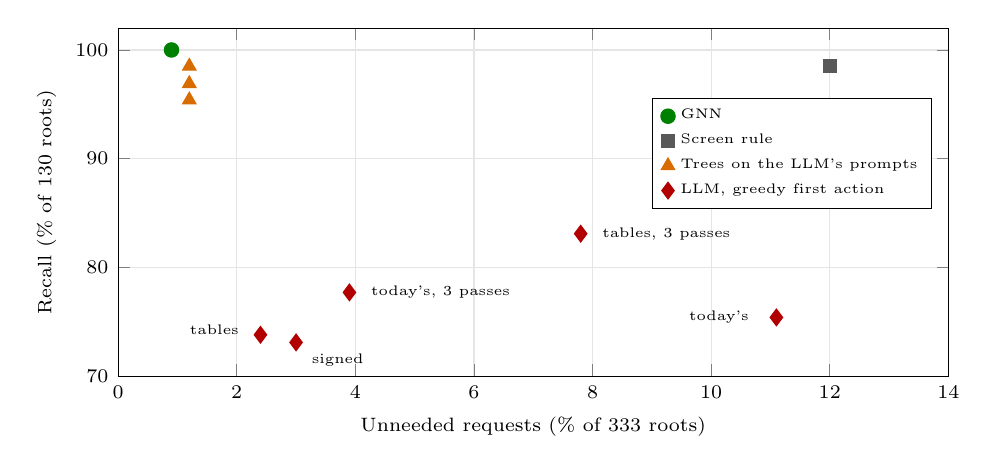
\begin{tikzpicture}
        \begin{axis}[
          width=\linewidth, height=6.0cm,
          xmin=0, xmax=14, ymin=70, ymax=102,
          xlabel={Unneeded requests (\% of 333 roots)},
          ylabel={Recall (\% of 130 roots)},
          label style={font=\scriptsize}, tick label style={font=\scriptsize},
          grid=major, grid style={gray!20},
          legend style={font=\tiny, at={(0.98,0.80)}, anchor=north east, cells={anchor=west}},
        ]
          \addplot[only marks, mark=*, mark size=2.6pt, color=green!50!black] coordinates {(0.9,100)};
          \addlegendentry{GNN}
          \addplot[only marks, mark=square*, mark size=2.3pt, color=gray!70!black] coordinates {(12.0,98.5)};
          \addlegendentry{Screen rule}
          \addplot[only marks, mark=triangle*, mark size=2.8pt, color=orange!85!black] coordinates {(1.2,95.4) (1.2,96.9) (1.2,98.5)};
          \addlegendentry{Trees on the LLM's prompts}
          \addplot[only marks, mark=diamond*, mark size=3pt, color=red!70!black] coordinates {(11.1,75.4) (3.0,73.1) (3.9,77.7) (2.4,73.8) (7.8,83.1)};
          \addlegendentry{LLM, greedy first action}
          \node[font=\tiny, anchor=east] at (axis cs:10.8,75.4) {today's};
          \node[font=\tiny, anchor=north west] at (axis cs:3.1,72.9) {signed};
          \node[font=\tiny, anchor=east] at (axis cs:2.2,74.3) {tables};
          \node[font=\tiny, anchor=west] at (axis cs:4.1,77.7) {today's, 3 passes};
          \node[font=\tiny, anchor=west] at (axis cs:8.0,83.1) {tables, 3 passes};
        \end{axis}
      \end{tikzpicture}
    \end{column}
    \begin{column}{0.4\textwidth}
      \footnotesize
      \begin{itemize}
        \setlength\itemsep{0.45em}
        \item Every one-pass LLM: \bad{73--75\%} recall, whatever the prompt.
        \item Best LLM: \textbf{83.1\%} at 7.8\% unneeded (tables, three passes at half the learning rate).
        \item Trees on the same prompt fields: \good{95--98.5\%} at 1.2\%.
        \item As a ranking the LLM reaches AUC 97.1\% at best (GNN 99.96\%). At the screen's recall it requests on 46--85\% of the roots that need none.
      \end{itemize}
    \end{column}
  \end{columns}
  \reportsource{S2 (\texttt{report.md}), S4. Every reading: appendix.}
\end{frame}

% 12
\begin{frame}{LLM Arm: What the Fine-Tune Learned}
  \scope{Requests on the test roots that need phasors, by family}
  \begin{center}
    \footnotesize
    \renewcommand{\arraystretch}{1.02}
    \begin{tabular}{lrrrrrrrr}
      \toprule
      & & \multicolumn{5}{c}{LLM, greedy} & & \\
      \cmidrule(lr){3-7}
      Family & Roots & today's & signed & today's $\times3$ & tables & tables $\times3$ & Trees & GNN \\
      \midrule
      Harmonic & 50 & 50 & 50 & 50 & 50 & 50 & 50 & 50 \\
      Unbalance & 30 & 28 & 28 & 26 & 28 & 28 & 28--29 & 30 \\
      HIF & 25 & 17 & 17 & 18 & 17 & 21 & 24--25 & 25 \\
      \rowcolor{red!6} HIF + bad meter & 25 & 3 & 0 & 7 & 1 & 9 & 22--24 & 25 \\
      \bottomrule
    \end{tabular}
  \end{center}
  \footnotesize
  \begin{itemize}
    \setlength\itemsep{0.25em}
    \item \textbf{One cue.} A depth-3 tree on the prompt fields reproduces 94--98\% of the LLM's request decisions. Its first split: the largest residual is a voltage magnitude; its second: that residual is not dwarfed by the largest branch multiplier.
    \item A voltage residual leads the list on 84 of the 130 roots that need phasors: every harmonic root, 29 of 30 unbalance, 5 of 25 HIF and no HIF behind a bad meter. With today's prompt the LLM requests on 100\% of the 10--20$\sigma$ voltage-meter probes and on 10\% of the bad power meters.
    \item The tables carry the information, since trees on them reach 98.5\%; the LLM's first action does not use it.
  \end{itemize}
  \reportsource{S1 (section 6), S4. Trees: largest class on the three prompt forms.}
\end{frame}

% 13
\begin{frame}{LLM Arm: Verdict for IEEE 14}
  \small
  \begin{itemize}
    \setlength\itemsep{0.6em}
    \item \textbf{Closed as a classifier.} With this recipe the LLM is not a triage classifier, so no DAgger cell uses the LLM as the gate.
    \item \textbf{More passes trade one error for the other.} Today's prompt, three passes: unneeded requests 11.1\% $\to$ 3.9\%, recall 75\% $\to$ 78\%. Tables at half the learning rate: recall 83\%, unneeded 7.8\%.
    \item \textbf{The recipe is fragile here.} One three-pass run diverged at the peak learning rate and ranked worse than chance (AUC 28.8\%).
    \item \textbf{The prompt is not the limit.} Trees on the same fields reach 95--98.5\% recall at 1.2\% unneeded.
    \item \textbf{What stays meaningful:} the agent acting on the GNN's report, against the agent acting on the screen's report.
    \item \textbf{Not tried:} more training roots, a larger model, a reasoning trace before the decision.
  \end{itemize}
  \reportsource{S1 (sections 7--8), S4.}
\end{frame}

% 14
\begin{frame}{The GNN-Gated Evidence Profile}
  \begin{center}
  \begin{adjustbox}{max width=\textwidth}
  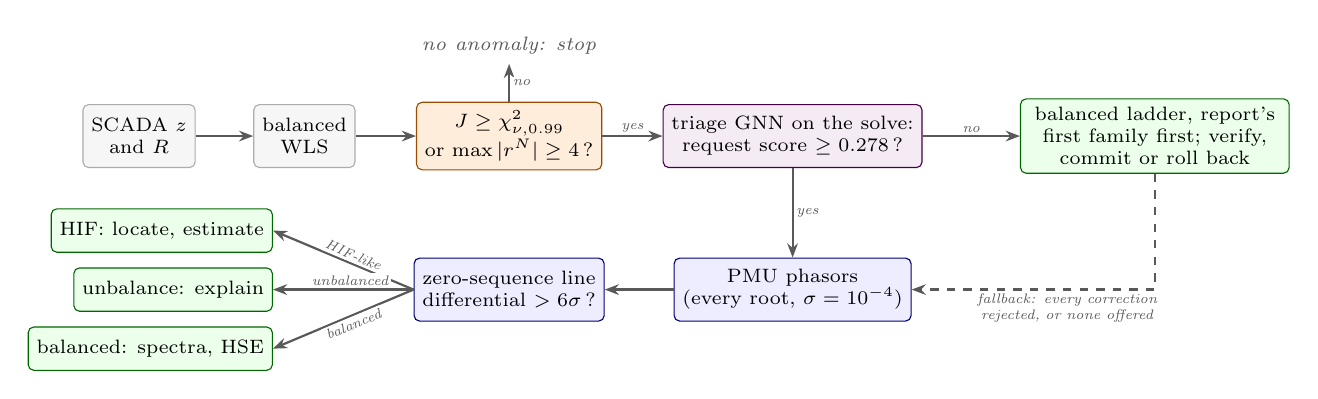
\begin{tikzpicture}[font=\scriptsize]
    \node[stage] (z) at (0,0) {SCADA $z$\\and $R$};
    \node[stage] (wls) at (2.1,0) {balanced\\WLS};
    \node[gate] (alarm) at (4.7,0) {$J\geq\chi^2_{\nu,0.99}$\\or $\max|r^N|\geq4$\,?};
    \node[gnn] (tri) at (8.3,0) {triage GNN on the solve:\\request score $\geq0.278$\,?};
    \node[font=\scriptsize\itshape, text=gray!70!black] (ok) at (4.7,1.15) {no anomaly: stop};
    \node[outc, text width=3.2cm] (ladder) at (12.9,0) {balanced ladder, report's\\first family first; verify,\\commit or roll back};
    \node[phys] (pmu) at (8.3,-1.95) {PMU phasors\\(every root, $\sigma=10^{-4}$)};
    \node[phys] (zs) at (4.7,-1.95) {zero-sequence line\\differential $>6\sigma$\,?};
    \node[outc, minimum height=0.55cm, anchor=east] (hif) at (1.7,-1.2) {HIF: locate, estimate};
    \node[outc, minimum height=0.55cm, anchor=east] (unb) at (1.7,-1.95) {unbalance: explain};
    \node[outc, minimum height=0.55cm, anchor=east] (har) at (1.7,-2.7) {balanced: spectra, HSE};
    \draw[arr] (z) -- (wls);
    \draw[arr] (wls) -- (alarm);
    \draw[arr] (alarm) -- node[lab, above] {yes} (tri);
    \draw[arr] (alarm) -- node[lab, right] {no} (ok);
    \draw[arr] (tri) -- node[lab, above] {no} (ladder);
    \draw[arr] (tri) -- node[lab, right] {yes} (pmu);
    \draw[arr, dashed] (ladder.south) |- node[lab, pos=0.68, below, text width=2.7cm, align=center] {fallback: every correction rejected, or none offered} (pmu.east);
    \draw[arr] (pmu) -- (zs);
    \draw[arr] (zs.west) -- node[lab, above, sloped, pos=0.45] {HIF-like} (hif.east);
    \draw[arr] (zs.west) -- node[lab, above, pos=0.45] {unbalanced} (unb.east);
    \draw[arr] (zs.west) -- node[lab, below, sloped, pos=0.45] {balanced} (har.east);
  \end{tikzpicture}
  \end{adjustbox}
  \end{center}
  \footnotesize
  \begin{itemize}
    \setlength\itemsep{0.2em}
    \item The report sits on the WLS ledger: request score, threshold, admission and the first balanced family. Nothing is added to the fault signatures.
    \item Same data contract as the screen profile: every root carries phasors and spectra. A classifier failure admits nothing, and the solve stands.
  \end{itemize}
  \reportsource{S1 (section 10), S5, S10 (\texttt{evidence\_profile.py}, \texttt{actions.py}).}
\end{frame}

% 15
\begin{frame}{Expert End to End: GNN Gate Against the Screen}
  \scope{Rule expert on the 160 development roots, 40 actions, one CPU}
  \begin{center}
    \footnotesize
    \renewcommand{\arraystretch}{1.18}
    \begin{tabular}{llrrrrr}
      \toprule
      Profile & Expert & Success & \makecell[r]{Phasors\\(unneeded)} & \makecell[r]{Spectra\\(unneeded)} & Mean steps & Wall time \\
      \midrule
      GNN-gated & baseline & 159/160 & 59 (3) & 18 (2) & 8.0 & \good{4.1 min} \\
      Screen & baseline & 159/160 & 59 (3) & 17 (1) & 8.6 & 10.0 min \\
      Screen & ledger and ranker & 160/160 & 58 (2) & 16 (0) & 7.9 & 9.4 min \\
      \bottomrule
    \end{tabular}
  \end{center}
  \small
  \begin{itemize}
    \setlength\itemsep{0.4em}
    \item The GNN's first report requests on all 40 roots that need phasors and on 1 of the 104 that need none (a multi-meter root at score 0.31).
    \item With the same expert, both profiles solve the same 159 roots and fail the same one. The GNN profile takes 2.4 times less wall time.
    \item The failing root is a parameter error whose true line ranks second among the multipliers (ratio 1.02). The screen's ledger names the right line; the baseline expert commits the wrong one. That is localization, not the request decision.
  \end{itemize}
  \reportsource{S1 (section 10), S6. ``Unneeded'' leaves out the 16 harmonic roots, where phasors come before the spectra for every teacher.}
\end{frame}

% 16
\begin{frame}{DAgger Cell with the GNN Gate}
  \scope{Gemma 4 12B, GNN-gated profile, baseline expert; the 160 development roots of the Oct 1 screen cell}
  \begin{columns}[T]
    \begin{column}{0.47\textwidth}
      \centering\footnotesize
      \renewcommand{\arraystretch}{1.08}
      \begin{tabularx}{\linewidth}{L{1.95cm}Y}
        \toprule
        Stage & Result \\
        \midrule
        D0 aggregate & 525 of 548 roots, 4,376 rows \\
        BC0 & 826 steps; validation loss 0.0048 \\
        Round 1 & 122 roots, 572 rows (label yield 86\%); R1 trained on 1,144 rows \\
        Round 2 & 122 roots, 537 rows; R2 trained; evaluation restarted after a preemption \\
        \bottomrule
      \end{tabularx}
    \end{column}
    \begin{column}{0.5\textwidth}
      \centering\footnotesize
      \renewcommand{\arraystretch}{1.12}
      \begin{tabular}{lrrr}
        \toprule
        Round 1 & Expert & BC0 & R1 \\
        \midrule
        Successes & 159 & 153 & \textbf{159} \\
        Invalid-action episodes & 0 & 10 & 3 \\
        False-commit episodes & 0 & 1 & 1 \\
        Loop episodes & 1 & 9 & 0 \\
        Mean steps & 8.01 & 9.16 & 8.02 \\
        \midrule
        Screen cell, Oct 1 & 160 & 152 & 158 \\
        \bottomrule
      \end{tabular}
    \end{column}
  \end{columns}
  \vspace{0.5em}
  \footnotesize
  \begin{itemize}
    \setlength\itemsep{0.2em}
    \item R1 matches the expert family by family; both miss only the misranked parameter root.
    \item BC0 loses 5 of the 8 HIF roots behind a bad meter, one topology root and the misranked root.
    \item The screen cell's round 2 fell to 156, every loss after balanced phasors on a voltage-meter suspicion.
  \end{itemize}
  \reportsource{S7 (\texttt{out/r1/round\_summary.json}, round-2 receipts), S8.}
\end{frame}

% 17
\begin{frame}{Trace Review: Leaks and Redundant Calls}
  \begin{columns}[T]
    \begin{column}{0.46\textwidth}
      \small
      \textbf{Family leaks: none found}
      \begin{itemize}
        \setlength\itemsep{0.3em}
        \item Every root carries phasors and spectra at the same sigma; no request answers by availability.
        \item The family-independent prompt fields are identical across the 13 families.
        \item Fault signatures come only from the agent's own diagnostics.
        \item The probes show no simulator-background effect.
      \end{itemize}
      \par\vspace{0.4em}
      HIF, harmonic, unbalance and healthy traces were already at the minimum the gates allow.
    \end{column}
    \begin{column}{0.51\textwidth}
      \small
      \textbf{Four changes for the next cell}
      \begin{enumerate}
        \setlength\itemsep{0.3em}
        \item \textbf{No family scores in the report.} Harmonic and unbalance differ from a bad voltage meter only through simulator artifacts.
        \item \textbf{No phasor re-acquisition} on a corrected child once they were tested.
        \item \textbf{One confirmation handoff} when a committed correction leaves the WLS quiet. Finalizing stays forbidden: an edit that only silences the alarm must not close the case.
        \item \textbf{Conditioned WLS inside the HIF estimate}, run by the environment, outside the agent's action budget.
      \end{enumerate}
    \end{column}
  \end{columns}
  \reportsource{S1 (section 12), S10 (commits 18c15f7, 11b7ad5).}
\end{frame}

% 18
\begin{frame}{Trimmed Contract: Old and New Traces}
  \scriptsize
  \renewcommand{\arraystretch}{1.12}
  \begin{tabularx}{\textwidth}{L{1.75cm}YY}
    \toprule
    Root & Before & Now \\
    \midrule
    HIF & WLS $\to$ phasors $\to$ NLM $\to$ HIF estimate $\to$ \bad{WLS} $\to$ finalize & WLS $\to$ phasors $\to$ NLM $\to$ HIF estimate (conditioned WLS inside) $\to$ finalize \\
    Meter, parameter or topology & WLS $\to$ context $\to$ correct $\to$ WLS $\to$ commit $\to$ \bad{context} $\to$ handoff & WLS $\to$ context $\to$ correct $\to$ WLS $\to$ commit $\to$ confirmation handoff \\
    HIF + bad meter & \ldots{} HIF estimate $\to$ \bad{WLS} $\to$ \ldots{} commit $\to$ \bad{context} $\to$ handoff & \ldots{} HIF estimate $\to$ \ldots{} commit $\to$ confirmation handoff \\
    \bottomrule
  \end{tabularx}
  \par\vspace{0.4em}
  \begin{center}
    \footnotesize
    \renewcommand{\arraystretch}{1.0}
    \begin{tabular}{lrrrr}
      \toprule
      160 development roots & \multicolumn{2}{c}{GNN-gated, baseline expert} & \multicolumn{2}{c}{Screen, ledger and ranker} \\
      \cmidrule(lr){2-3}\cmidrule(lr){4-5}
      & Before & Now & Before & Now \\
      \midrule
      Successes & 159 & 159 & 160 & 160 \\
      Tool calls & 1,282 & \good{1,161} & 1,256 & \good{1,137} \\
      Calls per HIF root & 6 & 5 & 6 & 5 \\
      Calls per HIF + bad meter root & 11.4 & 9.1 & 11.0 & 9.1 \\
      Calls per single balanced fault & 7 & 6 & 7 & 6 \\
      \bottomrule
    \end{tabular}
  \end{center}
  \reportsource{S6 (expert end-to-end runs before and after), S1 (section 12). Harmonic, unbalance and healthy roots are unchanged at 6, 4 and 2 calls.}
\end{frame}

% 19
\begin{frame}{Open Problems}
  \small
  \begin{itemize}
    \setlength\itemsep{0.55em}
    \item \textbf{Misranked parameter root.} The baseline expert commits the wrong line when the true one ranks second. The ledger teacher solves it in 6 calls; the GNN profile needs that ranking without the screen's refits.
    \item \textbf{Classifier false admissions.} A multi-meter root at the first WLS (score 0.31) and a meter-plus-topology child after its fix (0.40) each cost phasor and spectra calls.
    \item \textbf{No admission and nothing to try.} The episode ends in a handoff rather than a phasor request: the fallback needs a rejected correction, or a context that offered nothing.
    \item \textbf{One network.} The GNN is trained on IEEE 14 only, and its zero-shot IEEE 57 recall is 50\%.
    \item \textbf{Corpus format.} Topology roots are the only ones on the node-breaker operator model. The features neutralize it; one operator model for all roots would remove it.
  \end{itemize}
  \reportsource{S1 (sections 7, 8, 10 and 12), S6.}
\end{frame}

% 20
\begin{frame}{Next Experiments}
  \begin{enumerate}
    \setlength\itemsep{0.65em}
    \item \textbf{Finish round 2.} R2 against R1, and against the screen cell's R2 (156), on the same 160 roots.
    \item \textbf{Next cell on the trimmed contract.} The settings are ready; it needs about a day of GPU time.
    \item \textbf{A multi-network GNN.} IEEE 57 and 118 roots of every family, then leave-one-network-out.
    \item \textbf{Balanced localization without the screen.} Carry the ledger's candidate ranking into the parameter route.
    \item \textbf{One operator model for all roots}, to remove the last corpus-format cue.
  \end{enumerate}
\end{frame}

\appendix
% 21
\begin{frame}{Appendix: Every Request Reading on the Test Split}
  \scriptsize
  \renewcommand{\arraystretch}{0.92}
  \begin{center}
  \begin{tabular}{llrrrr}
    \toprule
    Classifier & Reading & AUC & Recall & Unneeded & Balanced pick true \\
    \midrule
    LLM, today's, 1 pass & greedy & -- & 75.4\% & 11.1\% & 66.0\% \\
    LLM, signed, 1 pass & greedy & -- & 73.1\% & 3.0\% & 82.1\% \\
    LLM, today's, 3 passes & greedy & -- & 77.7\% & 3.9\% & 80.5\% \\
    LLM, tables, 1 pass & greedy & -- & 73.8\% & 2.4\% & 83.3\% \\
    LLM, tables, 3 passes, half rate & greedy & -- & 83.1\% & 7.8\% & 76.4\% \\
    \midrule
    LLM, today's, 1 pass & probability & 91.5\% & 100\% & 85.3\% & 77.4\% \\
    LLM, signed, 1 pass & probability & 95.6\% & 99.2\% & 75.7\% & 85.2\% \\
    LLM, today's, 3 passes & probability & 94.7\% & 99.2\% & 55.3\% & 84.3\% \\
    LLM, tables, 1 pass & probability & 97.1\% & 100\% & 45.6\% & 85.8\% \\
    LLM, tables, 3 passes, half rate & probability & 95.7\% & 100\% & 49.2\% & 85.2\% \\
    \midrule
    Trees, today's prompt & largest class & -- & 95.4\% & 1.2\% & 96.2\% \\
    Trees, signed prompt & largest class & -- & 96.9\% & 1.2\% & 94.7\% \\
    Trees, tables prompt & largest class & -- & 98.5\% & 1.2\% & 96.2\% \\
    Trees, today's prompt & threshold & 99.85\% & 100\% & 13.5\% & 96.5\% \\
    Trees, signed prompt & threshold & 99.76\% & 100\% & 6.3\% & 95.9\% \\
    Trees, tables prompt & threshold & 99.9\% & 100\% & 3.0\% & 97.5\% \\
    \midrule
    GNN, residual-only & threshold & 99.96\% & 100\% & 0.9\% & 96.5\% \\
    \bottomrule
  \end{tabular}
  \end{center}
  \reportsource{S2, S1 (section 6). Thresholds reach the screen's calibration recall (99.3\%): 0.003 to 0.008 for the LLM's probability. Left out: the diverged run (signed, 3 passes; AUC 28.8\%).}
\end{frame}

% 22
\begin{frame}{Appendix: LLM Fine-Tunes}
  \footnotesize
  \renewcommand{\arraystretch}{1.05}
  \begin{center}
  \begin{tabularx}{\textwidth}{L{3.3cm}YL{1.9cm}}
    \toprule
    Run & Validation loss per answer token, every 128 steps & Scored \\
    \midrule
    Today's, 1 pass & 0.0356, 0.0335, 0.0336, 0.0361 (step 509) & step 256 \\
    Signed, 1 pass & 0.0362, 0.0325, 0.0456, 0.0232 (step 509) & step 509 \\
    Tables, 1 pass & 0.0549, 0.0331, 0.0212, 0.0201 (step 509) & step 509 \\
    Today's, 3 passes & 0.0331 \ldots{} 0.0260 (step 1,527); lowest 0.0241 & step 1,408 \\
    Signed, 3 passes & \bad{2.9063} at step 128, then 0.0765 \ldots{} 0.0482 & diverged \\
    Tables, 3 passes, half rate & between 0.023 and 0.038 throughout & step 640 \\
    \bottomrule
  \end{tabularx}
  \end{center}
  \small
  \begin{itemize}
    \setlength\itemsep{0.3em}
    \item 2.4 GPU hours per pass on an RTX PRO 6000. An answer is 19 to 21 tokens and one of them carries the decision: 0.033 per token is about 0.65 nats per decision.
    \item The signed three-pass run's training loss jumped above 8 at steps 82--86, near the peak learning rate. Its adapter requests on none of the 130 roots that need phasors.
    \item The half-rate run (5e-5) trained without a spike. Preempted runs resumed from their newest checkpoints.
  \end{itemize}
  \reportsource{S1 (section 6), S4.}
\end{frame}

% 23
\begin{frame}{Appendix: Sources}
  \scriptsize
  \begin{itemize}
    \setlength\itemsep{0.15em}
    \item[S1] \texttt{docs/classifier\_triage\_plan\_20261004.md}: plan, decisions, stage 0 to stage 2, contract changes (sections 1--12).
    \item[S2] \texttt{output/classifier\_triage\_20261004/ieee14/}: \texttt{report.md}, \texttt{benchmark.json}, probes, \texttt{transfer\_look\_ieee57.md}.
    \item[S3] \texttt{output/classifier\_triage\_20261004/ieee14\_location/}: held-out location study.
    \item[S4] \texttt{output/classifier\_triage\_20261004/llm}, \texttt{llm\_results/}; jobs in \texttt{research/hpc/classifier\_triage\_20261004/}.
    \item[S5] \texttt{research/classifier\_triage/} (\texttt{features.py}, \texttt{model.py}, \texttt{runtime.py}); export \texttt{psse\_env/oracle/models/triage\_gnn\_ieee14\_20261004}.
    \item[S6] \texttt{output/classifier\_triage\_20261004/e2e/}: expert end-to-end runs; \texttt{\_v2} runs after the trimmed contract.
    \item[S7] Cluster cell \texttt{research\_full\_pipeline\_20261007\_classifier}: \texttt{out/r1/round\_summary.json}, round-2 receipts.
    \item[S8] Cluster cell \texttt{research\_full\_pipeline\_20261001\_ranked}: \texttt{out/pipeline\_summary.json}.
    \item[S9] \texttt{docs/slides/weekly\_update\_20261002.tex} and \texttt{output/hypothesis\_ranking\_20260930/screen\_cost/}: screen cost.
    \item[S10] \texttt{psse\_env/evidence\_profile.py}, \texttt{actions.py}, \texttt{transactional\_env.py}, \texttt{oracle/diagnostics\_expert.py} (commits 18c15f7, 11b7ad5).
  \end{itemize}
\end{frame}

\end{document}
